\documentclass[usenames,dvipsnames, 9pt]{beamer}
\usepackage{amsmath,amsfonts,amssymb}
\usepackage{mathtools}
\usepackage{etex} %for Windows
\usepackage[utf8]{inputenc}
\usepackage[english, russian]{babel} 
%\usepackage{microtype}			% Better interword spacing and additional kerning.
\usepackage{ellipsis}			% Adjusted space with \dots between two words.
\usepackage{graphicx}
\usepackage{pstricks}

\usepackage{xcolor}


\usepackage{changepage}

\usepackage{algorithm}
\usepackage{algpseudocode}
%\usepackage[]{algorithm2e}
%\usepackage{algorithmic}

%\usepackage{tcolorbox}


\usepackage{caption}
\usepackage{subcaption}
%\usepackage{stackengine}


\usepackage{tikz}
\usetikzlibrary{tikzmark,calc}
\usetikzlibrary{positioning, backgrounds}
\usetikzlibrary{arrows, chains, matrix, scopes, patterns, shapes, fit}
\usetikzlibrary{mindmap,trees,shadows}
\usetikzlibrary{decorations.pathreplacing}
%\usetikzlibrary{crypto.symbols}

\usepackage{pgfplots}

\pgfmathdeclarefunction{gauss}{2}{%
	\pgfmathparse{1/(#2*sqrt(2*pi))*exp(-((x-#1)^2)/(2*#2^2))}%
}


\tikzset{
	invisible/.style={opacity=0},
	visible on/.style={alt={#1{}{invisible}}},
	alt/.code args={<#1>#2#3}{%
		\alt<#1>{\pgfkeysalso{#2}}{\pgfkeysalso{#3}} % \pgfkeysalso doesn't change the path
	},
}

\newcommand\strikeout[2][]{%
	\begin{tabular}[b]{@{}c@{}} 
		\makebox(0,0)[cb]{{#1}} \\[-0.2\normalbaselineskip]
		\rlap{\color{Orange}\rule[0.5ex]{\widthof{#2}}{1.5pt}}#2
\end{tabular}}

\newcommand\Fontvi{\fontsize{11}{13.2}\selectfont}

\usepackage{listings} % for C++ code

\usepackage{braket}
%\usepackage[braket, qm]{qcircuit}



\usepackage[T1]{fontenc}
%\usepackage[sfdefault,scaled=.85]{FiraSans}
%\usepackage{newtxsf}
%\usepackage[nomap]{FiraMono}





\usefonttheme[onlymath]{serif}
\renewcommand\sfdefault{cmbr}

\renewcommand{\bfdefault}{sb}

\definecolor{CharCoalDark}{RGB}{13, 16, 19}
\definecolor{Orange}{RGB}{255, 165,0}
\definecolor{DarkOrange}{RGB}{255, 165,0}
\definecolor{LightSalmon}{RGB}{255, 160, 122}
\definecolor{LeafGreen}{RGB}{34, 139,  34}
\definecolor{Coral}{RGB}{255, 127, 80}
\definecolor{DarkTurquoise}{RGB}{0, 206, 209}

%\newtheorem{defRus}{Определение}
%\newtheorem{thmRus}{Теорема}
%s\newtheorem{corRus}{Следствие}


\setbeamercolor{background canvas}{bg=CharCoalDark}

\setbeamerfont{title}{series=\bfseries}
\setbeamercolor{title}{fg=Orange}
\setbeamercolor{section in toc}{fg=white}
\setbeamercolor{frametitle}{fg=Orange}
\setbeamercolor{normal text}{fg=white}
%\setbeamercolor{normal text}{fontsize=12pt}
\setbeamercolor{itemize item}{fg=Orange}
\setbeamercolor{enumerate item}{fg=Orange}
\setbeamercolor{enumerate item item}{fg=Orange}
\setbeamercolor{itemize item item}{fg=Orange}
\setbeamercolor{enumerate item}{fg=Orange}
\setbeamercolor{block title}{bg=DarkOrange,fg=white}
\setbeamerfont{block title}{series=\bfseries}

\setbeamertemplate{itemize item}[circle]
\setbeamertemplate{eumerate subitem}{\color{Orange}[$\checkmark$]}
\setbeamertemplate{itemize subitem}{\color{Orange}\Large$\textbullet$}
\setbeamertemplate{itemize subitem}{\color{Orange} \tiny $\blacksquare$}

% footnote without a marker
\newcommand\blfootnote[1]{%
	\begingroup
	\renewcommand\footnoterule{}
	\renewcommand\thefootnote{}\footnote{#1}%
	\addtocounter{footnote}{-1}%
	\endgroup
}

\newcommand*{\Scale}[2][4]{\scalebox{#1}{\ensuremath{#2}}}%

\newcommand\Item[1][]{%
	\ifx\relax#1\relax  \item \else \item[#1] \fi
	\abovedisplayskip=0pt\abovedisplayshortskip=0pt~\vspace*{-\baselineskip}}

\pgfdeclareradialshading{ring}{\pgfpoint{0cm}{0cm}}%
{rgb(0cm)=(1,1,1);
	rgb(0.7cm)=(1,1,1);
	rgb(0.719cm)=(1,1,1);
	rgb(0.72cm)=(0.975,0,0);
	rgb(0.9cm)=(1,1,1)}

\usepackage[absolute,overlay]{textpos} %to clip to a corner
\newcommand\FrameText[1]{%
	\begin{textblock*}{\paperwidth}(\textwidth-35pt, 10 pt)
		\raggedright #1\hspace{.5em}
\end{textblock*}}

\makeatletter
\let\save@measuring@true\measuring@true
\def\measuring@true{%
	\save@measuring@true
	\def\beamer@sortzero##1{\beamer@ifnextcharospec{\beamer@sortzeroread{##1}}{}}%
	\def\beamer@sortzeroread##1<##2>{}%
	\def\beamer@finalnospec{}%
}
\makeatother

\AtBeginSection[]
{
	\begin{frame}<beamer>
		\frametitle{Outline}
		\tableofcontents[currentsection]
	\end{frame}
}


%\institute{ENS Lyon}
\author{Elena Kirshanova \\ [10pt]
}
\titlegraphic{
	
	%
\includegraphics[width=2.5cm]{stayhome}%
	%\includegraphics[width=4.0cm]{ens_logo_gray}
}
\title{\Huge Cryptographic Hash Function}

\date{ Course ``Information and Network Security'' \\ 	
	Lecture 6 \\ \today }


\setbeamertemplate{navigation symbols}{} %removes navigation

% proper highlightling of a code-snippet
\lstset{language=C++,
	keywordstyle=\color{magenta},
	stringstyle=\color{Goldenrod},
	commentstyle=\color{gray},
	breaklines=false,
	%morecomment=[l][\color{magenta}]{\#}
}

%\setlength{\parskip}{8pt}
% ==================================================================
% Definitions for this paper
% ==================================================================
\mathchardef\hyphen="2D

\usepackage{multirow}
\usepackage{multicol} % For multiple coloumn environments
%\usepackage{stmaryrd} % For set brackets
% \setlength{\columnsep}{15pt} % Defining the coloumn seperation
% \setlength{\columnseprule}{1pt} % Place a line between coloumns
% \newcommand{\tab}{\hspace*{2em}}

%subscripts

\newcommand*\SmallTextScript[2]{{\mathchoice{\displaystyle #2}
		{\textstyle #2}%dito
		{\scalebox{#1}{\ensuremath{\scriptstyle #2}}}%
		{\scalebox{#1}{\ensuremath{\scriptscriptstyle #2}}}%
}}


% ADVERSARIES AND SUCH
\newcommand*{\poly}{\ensuremath{\mathrm{poly}}}
\newcommand*{\eps}{\ensuremath{\varepsilon}}
\newcommand*{\alg}{\ensuremath{\mathcal{A}}}

% GROUPS/DISTRIBUTIONS/SETS/LISTS
\newcommand{\N}{{{\mathbb N}}}
\newcommand{\Z}{{{\mathbb Z}}}
\newcommand*{\IZ}{\ensuremath{\mathbb{Z}}}
\newcommand*{\IN}{\ensuremath{\mathbb{N}}}
\newcommand*{\IQ}{\ensuremath{\mathbb{Q}}}
\newcommand{\R}{{{\mathbb R}}}
\newcommand*{\IR}{{{\mathbb R}}}
\newcommand{\Zp}{\Z_p} % Integers modulo p
\newcommand{\Zq}{\Z_qs} % Integers modulo q
\newcommand{\Zn}{\ints_N} % Integers modulo N
\newcommand{\F}{\ensuremath{\mathbb{F}}}
\newcommand{\CC}{\ensuremath{\mathbb{C}}}

\newcommand{\ord}{\ensuremath{\mathrm{ord}}}

\newcommand{\GF}{\ensuremath{\mathbb{F}_2}}
\newcommand{\GFn}{\ensuremath{\mathbb{F}^n_2}}

%%% ALGORITHMS/PROCEDURES %%%
\newcommand{\Dec}{\textsf{Dec}}
\newcommand{\Enc}{\textsf{Enc}}
\newcommand{\KeyGen}{\textsf{KeyGen}}
\newcommand{\Gen}{\textsf{Gen}}
\newcommand{\MAC}{\textsf{MAC}}
\newcommand{\sk}{\textsf{sk}}
\newcommand{\pk}{\textsf{pk}}
\newcommand{\mesS}{\ensuremath{\mathcal{M}}}
\newcommand{\keyS}{\ensuremath{\mathcal{K}}}
\newcommand{\cipS}{\ensuremath{\mathcal{C}}}
\newcommand{\tagS}{\ensuremath{\mathcal{T}}}
\newcommand{\nonceS}{\ensuremath{\mathcal{N}}}
\newcommand{\mactag}{\textsf{tag}}
\newcommand{\Hash}{\ensuremath{\mathcal{H}}}
\newcommand{\EID}{\ensuremath{\mathtt{EphID}}}

\newcommand{\rem}{\ensuremath{\mathrm{rem}}}

\newcommand{\adv}{\ensuremath{\mathcal{A}}}

\newcommand{\LWE}{\mathsf{LWE}}
\newcommand{\DCP}{\mathsf{DCP}}
\newcommand{\EDCP}{\mathsf{EDCP}}
\newcommand{\UEDCP}{\mathsf{U \text{-} EDCP}}
\newcommand{\GEDCP}{\mathsf{G \text{-} EDCP}}



%% Landau and proba
\newcommand{\bigO}{\mathcal{O}}
\newcommand*{\OLandau}{\bigO}
\newcommand*{\WLandau}{\Omega}
\newcommand*{\xOLandau}{\widetilde{\OLandau}}
\newcommand*{\xWLandau}{\widetilde{\WLandau}}
\newcommand*{\TLandau}{\Theta}
\newcommand*{\xTLandau}{\widetilde{\TLandau}}
\newcommand{\smallo}{o} %technically, an omicron
\newcommand{\wLandau}{\omega}
\newcommand{\negl}{\mathrm{negl}}
\newcommand*\PROB\Pr 
\DeclareMathOperator*{\EXPECT}{\mathbb{E}}
\DeclareMathOperator*{\VARIANCE}{\mathbb{V}}
\DeclareMathOperator*{\LOGBIAS}{\mathbb{LB}}

\newcommand{\supp}{\ensuremath{\mathsf{sup}}}
\newcommand{\Distr}{\ensuremath{\mathcal{D}}}

% Lattices

% \newcommand{\coset}{\Lambda} % Lambda Lattice
% \newcommand{\cosetPerp}{\Lambda^{\bot}} % Lambda_Perp Lattice
% \newcommand{\gadget}{\textbf{G}} %Gaget matrix
% \newcommand{\mes}{\textbf{m}} %message vector
% \newcommand{\AMat}{\textbf{A}} %A matrices
% \newcommand{\BMat}{\textbf{B}} %B matrices
% \newcommand{\RMat}{\textbf{R}} %R matrices
% \newcommand{\HMat}{\textbf{H}} %H matrices
% \newcommand{\XMat}{\textbf{X}} %H matrices
% \newcommand{\mbar}{\bar{m}} %mBar dimension
% % \newcommand{\gauss}{\mathcal{D}} % gaussian distribution
% \newcommand{\Id}{\textbf{I}} % Identity matrix
% \newcommand{\er}{\textbf{e}} % gaussian distr. vectors
% % \newcommand{\cipher}{\textit{c}} % ciphertext
% \newcommand{\Olwe}{\mathcal{O}_{\textsf{LWE}}} %LWE oracle
% \newcommand{\OSample}{\mathcal{O}_{Sample}} %LWE oracle
% \newcommand{\SigmaB}{\boldsymbol{\Sigma}} %semi-deifinite matrix Sigma%
% % \newcommand{\mods}{\text{ mod}}


%Vectors and Matrices

\newcommand{\AMat}{\mathbf{A}} %A matrices
\newcommand{\BMat}{\mathbf{B}} %B matrices
\newcommand{\DMat}{\mathbf{D}} %Diagonal


\newcommand{\HMat}{\ensuremath{\mathbf{H}}}
\newcommand{\QMat}{\ensuremath{\mathbf{Q}}}
\newcommand{\Id}{\ensuremath{\mathbf{I}}}
\newcommand{\ZeroM}{\textbf{0}} % Zero matrix

\newcommand{\avec}{\ensuremath{\mathbf{a}}}
\newcommand{\bvec}{\ensuremath{\mathbf{b}}}
\newcommand{\cvec}{\ensuremath{\mathbf{c}}}
\newcommand{\evec}{\ensuremath{\mathbf{e}}}
\newcommand{\rvec}{\ensuremath{\mathbf{r}}}
\newcommand{\svec}{\ensuremath{\mathbf{s}}}
\newcommand{\tvec}{\ensuremath{\mathbf{t}}}
\newcommand{\vvec}{\ensuremath{\mathbf{v}}}
\newcommand{\zvec}{\ensuremath{\mathbf{z}}}
\newcommand{\xvec}{\ensuremath{\mathbf{x}}}
\newcommand{\yvec}{\ensuremath{\mathbf{y}}}
\newcommand{\uvec}{\ensuremath{\mathbf{u}}}
\newcommand{\zerovec}{\ensuremath{\mathbf{0}}}

\newcommand{\nth}{^{\mathrm{th}}}
\newcommand{\nd}{^{\mathrm{nd}}}

\newcommand{\RepMMT}{\ensuremath{\mathcal{R}_{\protect\SmallTextScript{0.70}{\texttt{MMT}}}}}
\newcommand{\RepBJMM}{\ensuremath{\mathcal{R}_{\protect\SmallTextScript{0.70}{\texttt{BJMM}}}}}
\newcommand{\XOR}{\ensuremath{\mathtt{3XOR}}}


% % % % % \newcommand{\mb}[1]{\mathbf{#1}} % does not compile otherwise
%%% Removed by Gotti; this is just asking to screw up with packages that (properly) define \mb (mathbold)

% \newcommand{\bL}{\|\bvec_1\|} % b1 length that appears way too often
% \newcommand{\dL}{\|\dvec_1\|} % b1 length that appears way too oftend

%Norms and Scalar products

\newcommand*\abs[1]{\left\lvert#1\right\rvert}
\newcommand*\norm[1]{\left\lVert#1\right\rVert}
\newcommand*\normalabs[1]{\lvert#1\rvert} 
\newcommand*\normalnorm[1]{\lVert#1\rVert}
\newcommand*\bignorm[1]{\bigl\lVert#1\bigr\rVert}
\newcommand*\bigabs[1]{\bigl\lvert#1\bigr\rvert}
\newcommand*\Bigabs[1]{\Bigl\lvert#1\Bigr\rvert}
\newcommand*{\ScProd}[2]{\ensuremath{\langle#1\mathbin{,}#2\rangle}} %Scalar Product
% \newcommand*{\ScProd}[2]{\ensuremath{\langle#1 \:{,}\:#2\rangle}} %Scalar Product
\newcommand*{\bigScProd}[2]{\ensuremath{\bigl\langle#1\mathbin{,}#2\bigr\rangle}} %Scalar Product
\newcommand*{\BigScProd}[2]{\ensuremath{\Bigl\langle#1\mathbin{,}#2\Bigr\rangle}} %Scalar Product
\newcommand{\dist}{\ensuremath{\text{dist}}}


%Some other math operators

\DeclareMathOperator{\Span}{Span} %span of vectors
\DeclareMathOperator{\vol}{\mathrm{vol}} %volume
\DeclareMathOperator{\LW}{LambertW} %Lambert W function
\DeclareMathOperator{\SD}{SD}
\DeclareMathOperator{\gradient}{grad}
\DeclareMathOperator{\TRACE}{Tr}
\newcommand*{\dDR}{\mathrm{d}} %de-Rham-Differential (the d in dx, dy, dz and so on)


%Lists
\renewcommand{\L}{\ensuremath{\mathcal{L}}}

\renewcommand{\P}{\ensuremath{\mathcal{P}}}

\newcommand*{\Lout}{\ensuremath{\L_{\mkern-0.5mu\protect\SmallTextScript{0.85}{\textup{out}}}}}
\newcommand*{\Sout}{\ensuremath{S_{\mkern-0.5mu\protect\SmallTextScript{0.85}{\textup{out}}}}}
\newcommand{\wt}{\ensuremath{\mathit{wt}}}


\newcommand*{\softO}{\widetilde{\bigO}}

\newcommand{\const}{\mathsf{c}} 


\newcommand{\transpose}{\mkern0.7mu^{\mathsf{ t}}}

%proper overline reduced by 1.5mu
\newcommand{\overbar}[1]{\mkern 1.5mu\overline{\mkern-1.5mu#1\mkern-1.5mu}\mkern 1.5mu}

\DeclareMathOperator{\erf}{erf} %error function
\DeclareMathOperator{\erfc}{erfc} %complementary error function
\newcommand{\Er}{\ensuremath{\mathrm{Er}}} %complementary error function


% LATTICES

\newcommand{\Lat}{\ensuremath{\mathcal{L}}}
\newcommand*{\Sphere}[1]{\ensuremath{\mathsf{S}^{#1}}}
%\DeclareMathOperator{\Conf}{Conf}
\newcommand{\Conf}{\mathcal{C}}

%Thick line for table
\setlength{\doublerulesep}{0pt}
\newcommand{\thickline}{\hline\hline\hline}


%circled text
\newcommand*\circled[1]{\tikz[baseline=(char.base)]{
    \node[shape=circle,draw,inner sep=0.3 pt] (char) {\scriptsize #1};}}


%Fix Algorithmicx package
\def\NoNumber#1{{\def\alglinenumber##1{}\State #1}\addtocounter{ALG@line}{-1}}

%For comments
\newcommand{\GColor}{ForestGreen}  %Damiens' color
\newcommand{\EColor}{MidnightBlue} %Elena's color

\newcommand*{\E}[1]{{\color{\EColor} #1} } 
\newcommand*{\G}[1]{{\color{\GColor} #1} } 

%Proper limit with the subscript underneath
% \newcommand{\Lim}[1]{\raisebox{0.5ex}{\scalebox{0.8}{$\displaystyle \lim_{#1}\;$}}}


%TIKZ dense dotted pattern

\pgfdeclarepatternformonly{my dots}{\pgfqpoint{-1pt}{-1pt}}{\pgfqpoint{2.0pt}{2.0pt}}{\pgfqpoint{2pt}{2pt}}%
{
	\pgfpathcircle{\pgfqpoint{0pt}{0pt}}{.35pt}
	\pgfpathcircle{\pgfqpoint{1pt}{1pt}}{.35pt}
	\pgfusepath{fill}
}


\tikzset{
	master/.style={
		execute at end picture={
			\coordinate (lower right) at (current bounding box.south east);
			\coordinate (upper left) at (current bounding box.north west);
		}
	},
	slave/.style={
		execute at end picture={
			\pgfresetboundingbox
			\path  (lower right)rectangle (upper left) ;
		}
	}
} %all defs
\begin{document}
	
\begin{frame}
	\titlepage
\end{frame}

\begin{frame}{Agenda}
	\Large 
	Last time:
	\begin{itemize}
		\item Achieve message integrity using MACs
		\item Construction of MACs from block ciphers. Example: CBC-MAC
	\end{itemize}
	\vspace{20pt}
	Today: \\
	
	Construct a more efficient MAC using {\color{Orange} hash functions (HMAC)}
\end{frame}

\begin{frame}{Cryptographic Hash Function: definition}
\Large
	A {\color{Orange}Hash function} is a \underline{pair} of polynomial time algorithms $(\Gen, \Hash)$:
	\begin{enumerate}
		\itemsep 7pt
		\item Probabilistic $\Gen: s \leftarrow \Gen(1^\lambda)$  
		\item Deterministic $\Hash_s: \{0,1\}^\star \rightarrow \{0,1\}^\ell$.
	\end{enumerate}
\pause
\vspace{10pt}
Most important property of $\Hash_s$ is {\color{Orange} collision resistant:}\\
Given $s$, there is no efficient adversary who can find two inputs $x, x' (x!=x')$ to $\Hash_s$ s.t.
\[
	\Hash_s(x) = \Hash(x')
\]

{\color{Orange} !} A ``hash'' function in general sense does not necessarily has this property. A {\color{Orange} cryptographic} hash function \underline{must} be collision resistant.\\[5pt]

There are \underline{many} collisions for $\Hash_s$, but it must be \underline{hard} to find any.
\end{frame}

\begin{frame}{Properties of cryptographic hash function}
\Large 
	{\color{Orange} I} Pre-image  resistance  (or one-wayness) \\[5pt]
	Given $(s, y)$\\
	Find $x$ s.t.\ $\Hash_s(x) =  y$ \\[5pt]
	{\color{Orange} A collision resistant hash function is also pre-image resistant}
	
	\pause 
	\vspace{20pt}
	{\color{Orange} II} $2\nd$ Pre-image  resistance \\[5pt]
	Given $(s, x)$\\
	Find $x'!=x$ s.t.\ $\Hash_s(x) =  \Hash_s(x')$ \\[5pt]
	{\color{Orange} A collision resistant hash function is also  $2\nd$  pre-image resistant}
	
	\vspace{20pt}
	\LARGE Conclusion: Collision resistance is the strongest requirement
\end{frame}

\begin{frame}{A word of caution: Exotic property of hash functions}
	\LARGE
	In BitCoind world the above three properties: \textbf{pre-image resistance}, \textbf{$2\nd$ pre-image resistance}, \textbf{collision resistance} may have other names: \textbf{``hiding''}, \textbf{``puzzle friendliness''}, \textbf{collision resistance}.\\[10pt]
	
	These are not special properties! BitCoin uses standardized cryptographic hash function (wait until the end of the lecture).
	
	\vfill
	See e.g. Section 1.1. in \url{https://d28rh4a8wq0iu5.cloudfront.net/bitcointech/readings/princeton_bitcoin_book.pdf?a=1}
\end{frame}

\begin{frame}{Generic attack on any hash function: birthday paradox}
\large 
	Remainder: Let $h_1, h_2, \ldots, h_n \in \{0,1\}^\ell$ be independent identically distributed bit strings. Then Birthday paradox says that
	\[
	\text{For } n = \bigO\left (\sqrt{ \abs{ \{0,1\}^\ell }} \right) = \bigO\left( 2^{\ell/2} \right) \quad  \Pr[\exists (i != j) \; : \; h_i = h_j] > 1/2.
	\]
	\pause
	Generic algorithm finds a collision in {\color{Orange} $\bigO(2^{\ell/2})$ } hash evaluations: \\
	\begin{enumerate}
		\itemsep 10pt
		\item Choose $ 2^{\ell/2}$ random bit strings (messages) $m_1, \ldots, m_{2^{\ell/2}}$ 
		\item  For each $m_i$ compute $h_i = \Hash_s(m_i)$, sort pairs to $(h_i, m_i)$ w.r.t.\ $h_i$
		\item  Find in the sorted list $h_i = h_j$. A collision $(m_i, m_j)$.
	\end{enumerate}			
	 Birthday paradox ensures that the above algorithm succeeds with constant success probability. 
	 \vfill
	\LARGE
	{\color{Orange} Conclusion:} Require  $\ell \geq 160$.
\end{frame}


\begin{frame}{Real world hash functions: historical overview}
\large
	\begin{enumerate}
		\itemsep7pt
		\item 1980s: MD4 (Message Digest) by R. Rivest.  {\color{Orange} $\ell = 128$} \\
		Status: {\color{Orange} Broken}. A collision can be found within seconds
		\pause
		\item 1990: MD5. {\color{Orange} $\ell = 128$} \\
		Status: {\color{Orange} Broken}. A collision can be found within seconds
		\pause
		\item 1995: SHA-1 (Secure Hash Algorithm 1) {\color{Orange} $\ell = 160$ } \\
		Status: {\color{Orange} Broken}. See \url{https://shattered.io/} for two PDFs with the same SHA-1 values. \\
		{\color{Orange} Caution:} may still be used by some systems (i.e., GIT).
		\pause
		\item 2001: SHA-2 (SHA-256, SHA-384, SHA-512). {\color{Orange} $\ell=256, 348, 512$} \\
		Status: {\color{Orange} Considered secure}
		\pause
		\item 2012: SHA-3 (Keccak). SHA-$3-224/256/348/512$. \\
		Status: {\color{Orange} Considered secure}
	\end{enumerate}
\pause
In Russia

	\begin{enumerate}
			\item GOST R 34.11-94 and GOST 34.311-95. {\color{Orange} $\ell = 256$} \\
			 Status: {\color{Orange} Depricated}  Collision  in $2^{105}$ time
			\item  GOST R 34.11-2012. Streebog {\color{Orange} $\ell = 256, 512$} \\
			 Status: {\color{Orange} Should be used in certified products}  
	\end{enumerate}
\end{frame}

\begin{frame}{Construction of a hash function: Merkle-Damg\aa rd paradigm}
\Large
Given a compression function (will be defined later) \[h: \keyS \times \mesS \rightarrow \keyS\]
Construct $\Hash: \mesS^\star \rightarrow \keyS$ \\

Let $m = (m_1, m_2, m_3 )$ of arbitrary length.
	\begin{figure}
		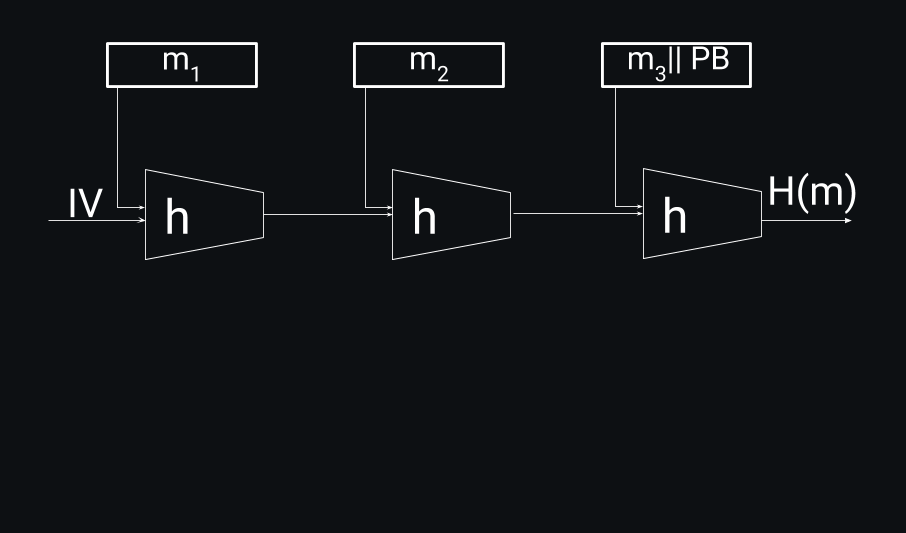
\includegraphics[width=0.9\textwidth]{MerkleDamgard}
	\end{figure}
\vspace{-60pt}
\textbf{IV} - Initial Value (fixed for given hash function) \\
\textbf{PB} - Padding Block $\left[100\ldots0 || \text{mes.\ length}\right]$. If \textbf{PB}  does not fit add another block

\end{frame}

\begin{frame}{Security of Merkle-Damg\aa rd construction}
\begin{figure}
	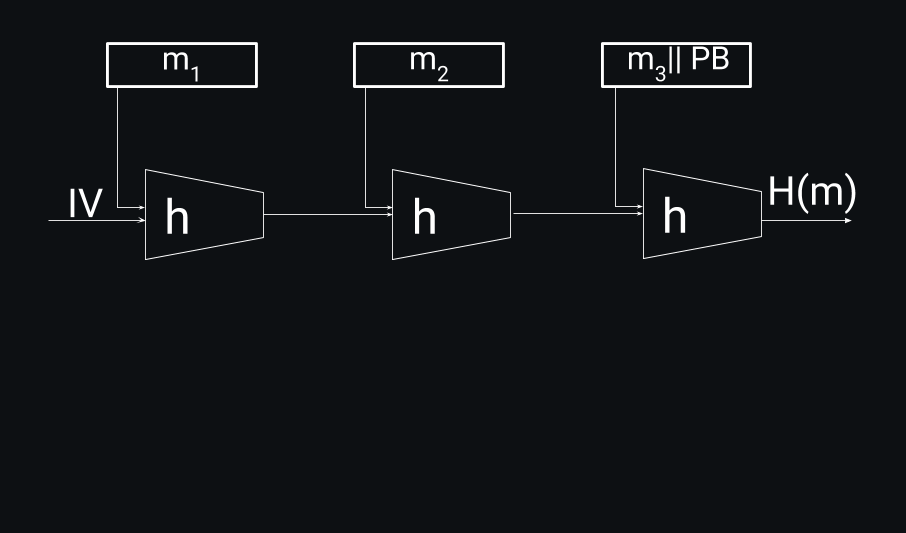
\includegraphics[width=0.9\textwidth]{MerkleDamgard}
\end{figure}
\vspace{-60pt}
\LARGE
{\color{Orange} Theorem:} If $h$ is collision resistant so is $H$.

\end{frame}

\begin{frame}{Construction of compressing function $h$}
\Large
	$\Enc: \keyS \times \{0,1\}^n \rightarrow  \{0,1\}^n$ -- a block-cipher.  \\{\color{Orange} Davies-Meyer construction:}
	\[
	h(H_{i}, m) = \Enc(H_i, m)\oplus H_i
	\]
	\begin{figure}
		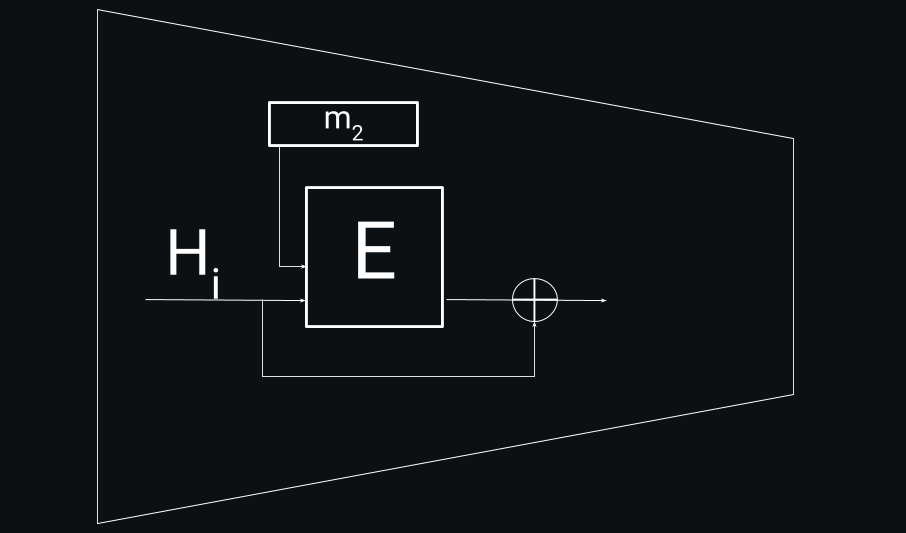
\includegraphics[width=0.7\textwidth]{DaviesMeyerCompression}
	\end{figure}

	{\color{Orange} Theorem (Informal):}  If $\Enc$ is a ``good'' cipher (i.e., $\Enc$ is a random permutation for fixed $k \in \keyS$),  then finding a collision $h(H, m) = h(H', m')$ takes $2^{n/2}$ evaluations of $(\Enc, \Dec)$.
	
\end{frame}

\begin{frame}{Example: SHA-256}
\Large 
In SHA-256 the compression function is:
	\begin{figure}
		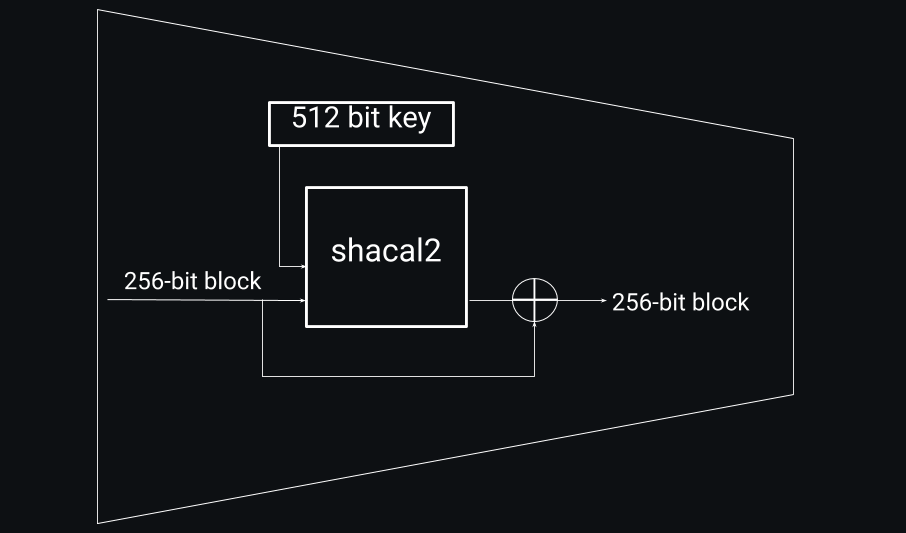
\includegraphics[width=0.9\textwidth]{SHA256}
	\end{figure}

 Merkle-Damg\aa rd construction is used to allow for arbitrary message length.

\end{frame}

\begin{frame}{Alternative construction of $h$}
	\Large
	{\color{Orange} Davies-Meyer construction:}
	\[
	h(H, m) = \Enc(H, m)\oplus H
	\]
	
	 {\color{Orange} Miyaguchi–Preneel  constriction:}
	 \[
	 h(H, m) = \Enc(H, m)\oplus H \oplus m
	 \]
	 
	 Other variants of combinations of $\Enc, H, m$ exist. Not all combination are secure! \\
	 GOST  Р 34.11-2012 (Streebog) uses Miyaguchi–Preneel.

\end{frame}

\begin{frame}{Sponge construction: SHA-3}
\large
SHA-3 (Keccak) is \underline{not} based on compression function. It is a {\color{Orange} Sponge} (рус.\ Губка) construction.

$P_0, \ldots P_{n-1}$ are derived from the input message.
$Z_0, Z_1, \ldots$ is the output

\begin{figure}
	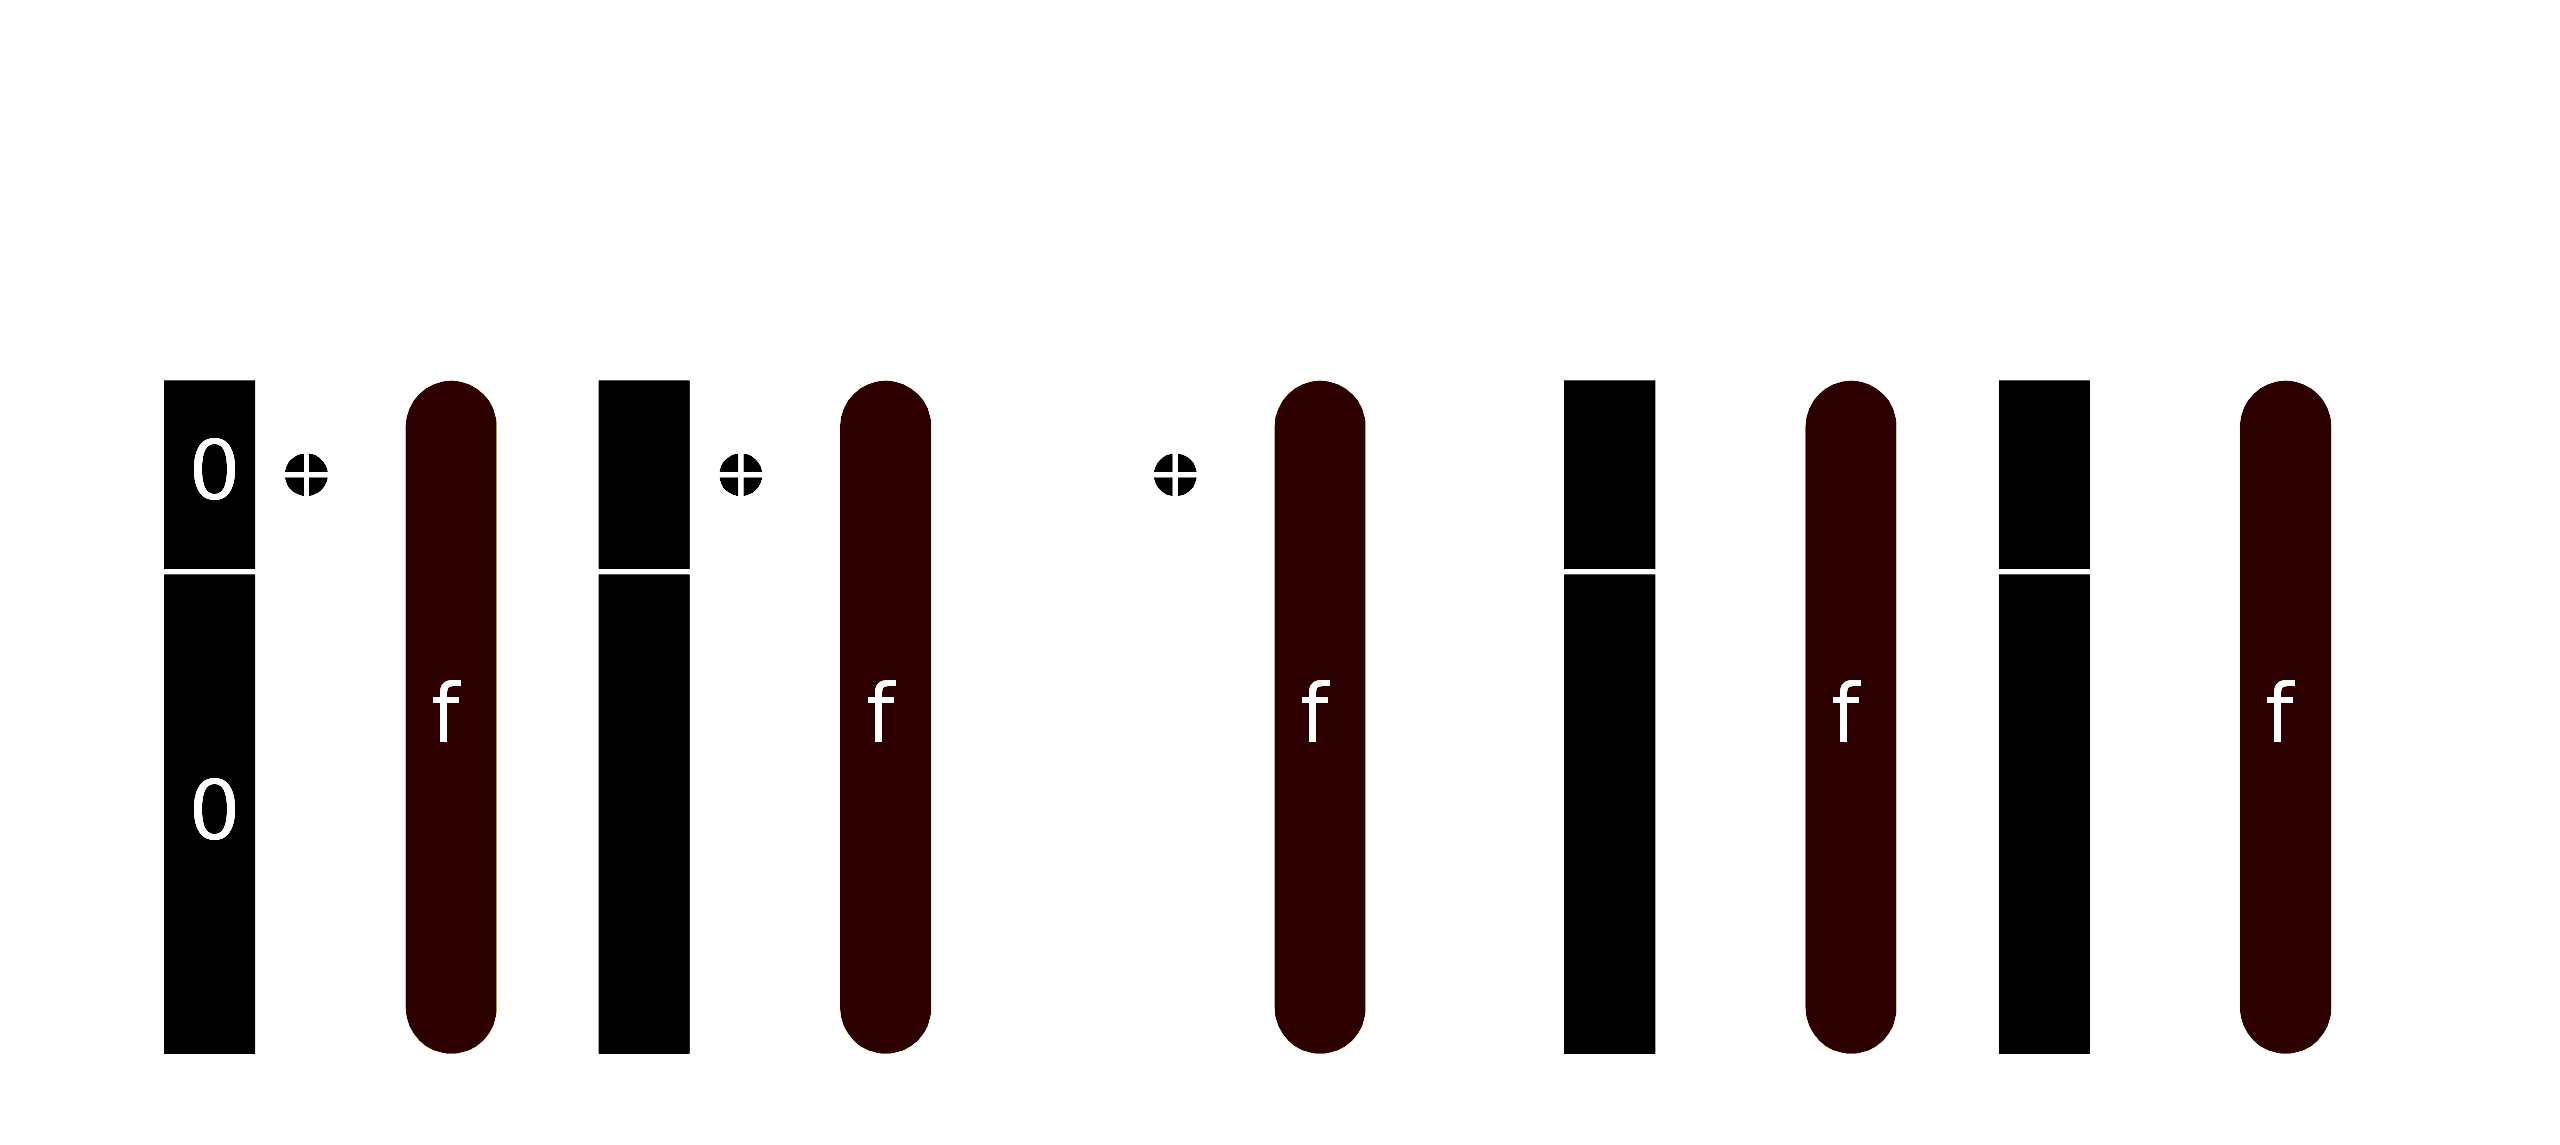
\includegraphics[width=0.9\textwidth]{SpongeConstruction}
\end{figure}

The block transformation $f$ is  a permutation consisting of 5 primitive function (small permutations, bitwise operations).


\vfill
\small
{\color{gray} CC Wikipedia} 

\end{frame}


\begin{frame}{Hash functions in BitCoin}
\Large
Basic concept in BitCoint: {\color{Orange} Proof of Work (PoW)} \\
Intuition: if a  user has computing power $\implies$ he should be able to prove it via doing some work\\
\vspace{15pt}
\begin{itemize}
	\itemsep 1em
	\item PoW introduced to crypto by Dwork \& Naor (1992) as a countermeasure against spam
	\item {\color{Orange} Idea:}  force users to solve some ``moderately hard'' puzzle (a solution should be fast to verify)
\end{itemize}
\end{frame}

\begin{frame}{Hash functions in BitCoin: constructing PoW}

\Large
Main primitive: cryptographic hash function $\Hash:\{0,1\}^\star \rightarrow \{0,1\}^\ell$  that takes $T(\Hash)$ time to evaluate

	\begin{center}
	\begin{tabular}{l c c c c}
		& Alice  & & Bob &  \\
		& Prover  & & Verifier &  \\
		& \multirow{5}{*}{
\includegraphics[scale=0.15]{Alice}} & & 
		\multirow{5}{*}{
\includegraphics[scale=0.15]{Bob}} & $x \in \{0,1\}^{\star}$   \\
		&  & \Huge $\xleftarrow{\mkern25mu x \mkern25mu}$ & &  \\ 
		Finds $s \in \{0,1\}^\star$   & & &  &  \\[-4pt]
		s.t.\ $\Hash(s||x)$ & & \Huge $\xrightarrow{\mkern25mu s \mkern25mu}$  &  &  \\
		starts with $n$ 0's & & &  &  Checks if \\
		  & & &  & $\Hash(s||x)$  has $n$ 0's\\
		{\color{Orange}  Time: $2^n T(\Hash) $} & & &  &  {\color{Orange}  Time: $T(\Hash) $}
	\end{tabular}
\end{center}

For a cryptographic hash function $\Hash$ Alice cannot do better than brute-force over $s$. This is a pre-image search. 
\end{frame}

\end{document}
